\documentclass[UTF8,fontset=none,10pt,a4paper]{ctexart}

\usepackage[left=17mm,right=17mm,top=20mm,bottom=19mm,headheight=21pt]{geometry}
\usepackage{fontspec}
\setmainfont{Noto Serif CJK SC}
\setsansfont{Noto Sans CJK SC}
\setmonofont[Scale=0.86]{DejaVu Sans Mono}
\setCJKmainfont{Noto Serif CJK SC}
\setCJKsansfont{Noto Sans CJK SC}
\setCJKmonofont{Noto Sans Mono CJK SC}

\usepackage[table,dvipsnames]{xcolor}
\definecolor{Ink}{HTML}{172033}
\definecolor{Muted}{HTML}{5F6B7A}
\definecolor{Navy}{HTML}{0B1F3A}
\definecolor{Blue}{HTML}{2563EB}
\definecolor{Sky}{HTML}{0EA5E9}
\definecolor{Cyan}{HTML}{06B6D4}
\definecolor{Green}{HTML}{059669}
\definecolor{Amber}{HTML}{D97706}
\definecolor{Red}{HTML}{DC2626}
\definecolor{Purple}{HTML}{7C3AED}
\definecolor{PaleBlue}{HTML}{EFF6FF}
\definecolor{PaleSky}{HTML}{ECFEFF}
\definecolor{PaleGreen}{HTML}{ECFDF5}
\definecolor{PaleAmber}{HTML}{FFFBEB}
\definecolor{PaleRed}{HTML}{FEF2F2}
\definecolor{Line}{HTML}{D8E0EA}
\definecolor{Paper}{HTML}{F7F9FC}

\usepackage{microtype}
\usepackage{setspace}
\setstretch{1.11}
\setlength{\parindent}{0pt}
\setlength{\parskip}{4.5pt}
\usepackage{enumitem}
\setlist{nosep,leftmargin=1.75em}
\usepackage{booktabs}
\usepackage{tabularx}
\usepackage{array}
\usepackage{longtable}
\usepackage{multirow}
\usepackage{makecell}
\usepackage{siunitx}
\sisetup{detect-all,group-separator={,},group-minimum-digits=4}
\usepackage{amsmath,amssymb,mathtools}
\usepackage{listings}
\usepackage{caption}
\usepackage{subcaption}
\usepackage{tikz}
\usetikzlibrary{arrows.meta,positioning,fit,calc,backgrounds,shapes.geometric,shadows.blur,matrix}
\usepackage{pgfplots}
\pgfplotsset{compat=1.18}
\usepackage[most]{tcolorbox}
\usepackage{titlesec}
\usepackage{fancyhdr}
\usepackage{lastpage}
\usepackage{hyperref}
\usepackage{xurl}

\hypersetup{
  colorlinks=true,
  linkcolor=Blue,
  urlcolor=Blue,
  citecolor=Blue,
  pdfauthor={qos\_storage\_sim experiment audit},
  pdftitle={连续满载下的需求感知带宽分配与 Adaptive Scheme B V2.1 落地指南},
  pdfsubject={Closed-loop traffic semantics, QoS allocation, and production migration}
}

\titleformat{\section}
  {\Large\bfseries\sffamily\color{Navy}}
  {\colorbox{Blue}{\textcolor{white}{\makebox[1.8em][c]{\thesection}}}}
  {0.7em}{}
\titleformat{\subsection}
  {\large\bfseries\sffamily\color{Navy}}
  {\thesubsection}{0.55em}{}
\titleformat{\subsubsection}
  {\normalsize\bfseries\sffamily\color{Ink}}
  {\thesubsubsection}{0.5em}{}
\titlespacing*{\section}{0pt}{1.35em}{0.65em}
\titlespacing*{\subsection}{0pt}{1.05em}{0.45em}

\pagestyle{fancy}
\fancyhf{}
\fancyhead[L]{\sffamily\small\color{Muted}需求感知带宽分配 · Adaptive Scheme B V2.1}
\fancyhead[R]{\sffamily\small\color{Muted}qos\_storage\_sim}
\fancyfoot[L]{\sffamily\footnotesize\color{Muted}2026-08-30 · 设计审计与生产迁移指南}
\fancyfoot[R]{\sffamily\footnotesize\color{Muted}\thepage\,/\,\pageref*{LastPage}}
\renewcommand{\headrulewidth}{0.4pt}
\renewcommand{\headrule}{\hbox to\headwidth{\color{Line}\leaders\hrule height \headrulewidth\hfill}}

\newcolumntype{Y}{>{\raggedright\arraybackslash}X}
\newcolumntype{C}{>{\centering\arraybackslash}X}
\newcolumntype{R}{>{\raggedleft\arraybackslash}X}
\renewcommand{\arraystretch}{1.22}
\captionsetup{font=small,labelfont={bf,sf,color=Navy},textfont={color=Muted}}

\newtcolorbox{verdictbox}[1][]{
  enhanced,breakable,colback=PaleBlue,colframe=Blue,boxrule=0pt,
  borderline west={3pt}{0pt}{Blue},arc=2mm,left=4mm,right=4mm,top=3mm,bottom=3mm,
  fonttitle=\bfseries\sffamily,title={结论},#1
}
\newtcolorbox{insightbox}[2][]{
  enhanced,breakable,colback=#2!7!white,colframe=#2,boxrule=0.65pt,
  arc=2mm,left=3.5mm,right=3.5mm,top=2.5mm,bottom=2.5mm,#1
}
\newtcolorbox{kpicard}[2][]{
  enhanced,colback=white,colframe=Line,boxrule=0.65pt,arc=2.5mm,
  left=3mm,right=3mm,top=2.5mm,bottom=2.5mm,
  drop fuzzy shadow,fonttitle=\bfseries\sffamily\color{Muted},title={#2},#1
}
\newcommand{\pill}[2]{\tikz[baseline=(X.base)]\node[rounded corners=4pt,inner xsep=5pt,inner ysep=2pt,fill=#1!12,text=#1,font=\sffamily\bfseries\footnotesize] (X) {#2};}
\newcommand{\good}{\textcolor{Green}{\bfseries ✓}}
\newcommand{\warn}{\textcolor{Amber}{\bfseries !}}
\newcommand{\bad}{\textcolor{Red}{\bfseries ×}}
\newcommand{\code}[1]{\texttt{\small #1}}
\newcommand{\pp}{\,pp}

\lstdefinestyle{modernpython}{
  language=Python,
  basicstyle=\ttfamily\footnotesize,
  keywordstyle=\color{Blue}\bfseries,
  commentstyle=\color{Green!75!black},
  stringstyle=\color{Purple},
  numbers=left,numberstyle=\tiny\color{Muted},numbersep=7pt,
  frame=single,rulecolor=\color{Line},backgroundcolor=\color{Paper},
  breaklines=true,showstringspaces=false,tabsize=2,
  xleftmargin=1.1em,framexleftmargin=0.8em,
  aboveskip=0.8em,belowskip=0.8em
}

\tikzset{
  flow/.style={draw=Line,fill=white,rounded corners=2mm,minimum height=9mm,
    text width=31mm,align=center,font=\sffamily\small,drop shadow},
  flowblue/.style={flow,draw=Blue!60,fill=PaleBlue},
  flowgreen/.style={flow,draw=Green!60,fill=PaleGreen},
  flowamber/.style={flow,draw=Amber!60,fill=PaleAmber},
  arrow/.style={-{Stealth[length=2.2mm]},thick,color=Muted},
  dashedarrow/.style={arrow,dashed,color=Sky}
}

\begin{document}

% --------------------------------------------------------------------------
% Cover
% --------------------------------------------------------------------------
\begin{titlepage}
\thispagestyle{empty}
\begin{tikzpicture}[remember picture,overlay]
  \fill[Navy] (current page.south west) rectangle (current page.north east);
  \fill[Blue,opacity=.22] ($(current page.north east)+(-18mm,-28mm)$) circle (54mm);
  \fill[Cyan,opacity=.17] ($(current page.south west)+(18mm,22mm)$) circle (50mm);
  \fill[Purple,opacity=.14] ($(current page.south east)+(-8mm,75mm)$) circle (39mm);
  \draw[white,opacity=.10,line width=.35pt,step=8mm]
    ($(current page.south west)+(0,18mm)$) grid ($(current page.north east)+(0,-18mm)$);
  \fill[Sky] ($(current page.north west)+(17mm,-19mm)$) rectangle ++(18mm,2mm);
\end{tikzpicture}

\vspace*{25mm}
{\sffamily\bfseries\color{Sky}\large SYSTEMS NOTE · 2026/08/30\par}
\vspace{13mm}
{\sffamily\bfseries\color{white}\fontsize{28}{35}\selectfont
连续满载下的\par
需求感知带宽分配\par}
\vspace{5mm}
{\sffamily\color{white!86}\fontsize{16}{22}\selectfont
为什么“盘侧不知道 10/30 GB/s”不必导致长期错配，\par
以及 Adaptive Admission Scheme B V2.1 如何从仿真走向生产\par}

\vspace{16mm}
\begin{tcolorbox}[enhanced,width=.89\textwidth,colback=Blue!24!Navy,
  colframe=Sky!55!Navy,boxrule=.8pt,arc=3mm,
  left=5mm,right=5mm,top=4mm,bottom=4mm]
{\sffamily\bfseries\color{white}\large 一句话结论}\par\smallskip
{\color{white!84}\large
磁盘无需读取“需求标签”也能在稳定细粒度流中形成 30/10 的长期服务；
真正需要需求感知的是有限 layer barrier 前的完整 coflow，而不是长期字节守恒。
新策略的收益是把更多请求推过 binary SLO 阈值，不是创造额外带宽。}
\end{tcolorbox}

\vfill
\begin{minipage}[t]{.29\textwidth}
  {\color{white!60}\sffamily\small SSU24 · SLO 增益}\par
  {\color{white}\sffamily\bfseries\fontsize{22}{26}\selectfont +27.10\pp}\par
  {\color{white!65}\small util $-0.25\pp$}
\end{minipage}\hfill
\begin{minipage}[t]{.29\textwidth}
  {\color{white!60}\sffamily\small SSU40 · SLO 增益}\par
  {\color{white}\sffamily\bfseries\fontsize{22}{26}\selectfont +32.45\pp}\par
  {\color{white!65}\small util $-0.03\pp$}
\end{minipage}\hfill
\begin{minipage}[t]{.29\textwidth}
  {\color{white!60}\sffamily\small SSU70 · SLO 增益}\par
  {\color{white}\sffamily\bfseries\fontsize{22}{26}\selectfont +21.54\pp}\par
  {\color{white!65}\small util $+1.92\pp$}
\end{minipage}

\vspace{14mm}
{\sffamily\color{white!55}\small
基于真实 \code{data} 请求画像 · 128 NPU · 16 层 · SSD40 / NPU50 · batch=1\par
正式策略：Adaptive Admission Scheme B V2.1（25 ms event-gated minimum spacing）}
\end{titlepage}

\pagenumbering{roman}
\begin{tcolorbox}[enhanced,colback=Paper,colframe=Line,boxrule=.5pt,arc=2mm,
  left=4mm,right=4mm,top=3mm,bottom=3mm]
\textbf{阅读说明。} 本报告把“需求”拆成需求标签、实际入队字节、长期服务率与 deadline
四个量；正式结果只引用已完成、输入指纹配对的实验。文中的 V2.1 是正式跑过
128-NPU 的新策略；编号更大的 deadline/barrier V3 只是已被当前数据淘汰的原型，
不会混入主结论。
\end{tcolorbox}
\tableofcontents
\clearpage
\pagenumbering{arabic}

% --------------------------------------------------------------------------
\section{决策摘要：不是 trace 或直觉的二选一}

\begin{verdictbox}
你的直觉\textbf{方向正确，但前提不完整}。当多个流都持续 backlogged，而调度器在相关
deadline 窗口内给了错误份额时，确实会产生 NPU bubble。可是，在当前闭环、按层释放的
连续 prefill 中，“请求需要 30 GB/s”并不等于磁盘入口存在一个永不变化的 30 GB/s
外部流。实际入队字节本身会携带需求比例，并被 compute/barrier 反压。工作保持的
Path0 FIFO 即使不知道需求标签，长期服务仍可能自然成为 30/10。
\end{verdictbox}

\begin{minipage}[t]{.32\textwidth}
\begin{kpicard}{你的想法成立之处}
\textcolor{Green}{\Large\bfseries ✓}\quad
有限 deadline 内，错误顺序或错误份额会让 barrier-critical 请求晚到，NPU 因而空等。
需求感知对 SLO 很重要。
\end{kpicard}
\end{minipage}\hfill
\begin{minipage}[t]{.32\textwidth}
\begin{kpicard}{当前 trace 的不同}
\textcolor{Blue}{\Large\bfseries $\circlearrowleft$}\quad
请求永远有后继，但 I/O 按层因果释放；高需求不是独立恒速注入器。队列由实际 block
字节和 barrier 状态共同塑形。
\end{kpicard}
\end{minipage}\hfill
\begin{minipage}[t]{.32\textwidth}
\begin{kpicard}{新策略真正做到的事}
\textcolor{Purple}{\Large\bfseries ⇧}\quad
根据完整 remaining manifest 保护一组可达标请求，把等待转移到有 SLO 余量的请求；
不改变 placement，也不突破 SSD40。
\end{kpicard}
\end{minipage}

\subsection{四个经常被混为一谈的“带宽”}

\rowcolors{2}{Paper}{white}
\begin{tabularx}{\textwidth}{>{\bfseries\sffamily}p{28mm} Y Y}
\toprule
量 & 定义 & 磁盘不知道它会怎样？\\
\midrule
Raw demand $D$ & 每层字节除以理想 compute window；表示完全隐藏 I/O 所需速率 & 不会自动按该标签分配；它只是控制器的计划输入\\
Actual offered work $A$ & 真正进入 SSD 队列的字节时间线 & 磁盘必然看见；队列中的字节比例本身编码了流量\\
Service $S$ & SSD 实际完成的字节与时间积分 & 工作保持系统中由队列、命令顺序与容量共同决定\\
Deadline success & 所有 SSU 的最后一块是否在 barrier 前到达 & 仅长期 $S/T$ 正确仍不够；需要需求/截止期感知\\
\bottomrule
\end{tabularx}
\rowcolors{2}{}{}

\begin{insightbox}[title={最终判断}]{Blue}
\textbf{如果你的目标是模拟真实的闭环满载 NPU pipeline：} 当前 trace 的基本类型是对的，
但有限 32-request prefix、2 s 测量窗和 queue drift 意味着“严格无限稳态”仍需更长循环验证。\par
\textbf{如果你的目标是模拟与 NPU 进度无关的 open-loop 10/30 GB/s 恒速流：}
当前 trace 不是那个模型，应另建固定 offered-rate 发生器。此时不是 trace “错误”，而是实验问题不同。
\end{insightbox}

% --------------------------------------------------------------------------
\section{先回答最常被问的问题：为什么换了策略，NPU 利用率几乎不动}
\label{sec:ceiling}

\begin{verdictbox}[title={一句话}]
\textbf{NPU 利用率不是策略能调的旋钮，它是“盘一共送出多少字节”的影子。}
在本仿真的工作保持（work-conserving）仲裁下，改变 CIR 只改变\textbf{字节送给谁}，
不改变\textbf{字节总量}，因此对总利用率是严格零和的。利用率的天花板由 placement
热点决定；策略的收益只能出现在\textbf{分布和 SLO} 上——而它确实拿到了。
\end{verdictbox}

本节是为第一次读这份报告的人写的。它用三步回答“为什么 Baseline 的利用率已经那么高、
新策略却提不动”，每一步都可以用本仓库的 JSON 结果手工复核。

\subsection{三分钟直觉：传送带、分料员和工人}

\begin{center}
\begin{tikzpicture}[node distance=7mm and 14mm]
  \node[flowamber,text width=33mm] (belt) {\textbf{传送带}\\SSD 总吞吐\\（每秒能送多少料）};
  \node[flow,right=of belt,text width=33mm,draw=Purple!60,fill=Purple!7] (qos)
    {\textbf{分料员}\\QoS / CIR 策略\\（决定先给谁）};
  \node[flowblue,right=of qos,text width=15mm,yshift=11mm] (w1) {工人 A};
  \node[flowblue,right=of qos,text width=15mm,yshift=-11mm] (w2) {工人 B};
  \draw[arrow] (belt) -- (qos);
  \draw[arrow] (qos.east) -- (w1.west);
  \draw[arrow] (qos.east) -- (w2.west);
  \node[below=9mm of qos,font=\small\sffamily,text=Muted,align=center,text width=95mm]
    {分料员可以让 A 先拿、B 后拿，\textbf{但他手上的料总量是传送带给的}。\\
     只要没人闲着等料，工人的总忙碌时间就和分料顺序无关。};
\end{tikzpicture}
\end{center}

NPU 是工人，SSD 是传送带，QoS 策略是分料员。要让“分料不均”真正压低总产能，必须存在
一条\textbf{浪费通道}：分给 A 的料 A 用不掉，\emph{而且}这份料被锁住、不能转给 B。

本仿真里这条通道是堵死的，原因见 \S\ref{subsec:zerosum}。所以分料员再聪明，也只能改变
\textbf{谁先拿到料}（$\Rightarrow$ 谁能赶上 deadline $\Rightarrow$ SLO），不能改变
\textbf{一共送出多少料}（$\Rightarrow$ 总利用率）。

\begin{insightbox}[title={术语速查：四个名字很像、含义完全不同的量}]{Blue}
\begin{tabularx}{\linewidth}{>{\bfseries\sffamily}p{34mm} Y}
\toprule
NPU 利用率 $U$ & 测量窗内 NPU 真正在算的时间占比。\textbf{本报告的主指标，但它是结果不是原因。}\\
SSD 利用率 $u_{ssd}$ & 盘在忙着搬数据的时间占比。反映盘有没有被喂饱。\\
Fleet raw demand $D$ & 若要让所有 NPU 一刻不停，盘侧总共需要的速率。本 workload 固定为
\textbf{2664.945 GB/s}，与 SSU 数量无关。\\
SLO 达成率 & 请求是否在 layer barrier 前拿到全部数据。\textbf{这才是策略能改的量。}\\
\bottomrule
\end{tabularx}
\end{insightbox}

\subsection{第一步：利用率是吞吐的影子（一条恒等式）}

NPU 只有拿到数据才能算。测量窗内盘一共送出 $N_{ssu}\cdot B_{ssd}\cdot u_{ssd}$ 的速率，
而“喂饱全部 NPU”需要 $D$，于是：

\begin{equation}
  \boxed{\;U \;=\; \frac{N_{ssu}\cdot B_{ssd}\cdot u_{ssd}}{D}\;}
  \qquad B_{ssd}=40\ \mathrm{GB/s},\quad D=2664.945\ \mathrm{GB/s}
  \label{eq:util-identity}
\end{equation}

\textbf{手算一遍 SSU24 Baseline：}$24\times 40\times 0.9094 \,/\, 2664.945 = 32.76\%$，
实测正是 $32.76\%$。下表把全部 17 次 128-NPU 正式运行代进去：

\rowcolors{2}{Paper}{white}
\begin{tabularx}{\textwidth}{p{37mm} C C C C C}
\toprule
策略 & SSU & $u_{ssd}$ & 式\eqref{eq:util-identity} 预测 & 实测 $U$ & 偏差\\
\midrule
baseline            & 16 & 0.9433 & 22.65\% & 22.64\% & $-0.02$\pp\\
baseline            & 24 & 0.9094 & 32.76\% & 32.76\% & $+0.00$\pp\\
current\_scheme\_b  & 24 & 0.8986 & 32.37\% & 32.38\% & $+0.01$\pp\\
admission\_v2\_25ms & 24 & 0.9037 & 32.55\% & 32.51\% & $-0.04$\pp\\
adaptive\_v2\_1\_25ms & 24 & 0.9037 & 32.55\% & 32.51\% & $-0.04$\pp\\
baseline            & 40 & 0.8591 & 51.58\% & 51.60\% & $+0.02$\pp\\
current\_scheme\_b  & 40 & 0.8586 & 51.55\% & 51.57\% & $+0.02$\pp\\
admission\_25ms     & 40 & 0.8589 & 51.57\% & 51.57\% & $+0.00$\pp\\
admission\_50ms     & 40 & 0.8603 & 51.65\% & 51.70\% & $+0.05$\pp\\
admission\_v2\_25ms & 40 & 0.8599 & 51.62\% & 51.66\% & $+0.03$\pp\\
adaptive\_v2\_1\_25ms & 40 & 0.8589 & 51.57\% & 51.57\% & $+0.00$\pp\\
baseline            & 70 & 0.8493 & 89.24\% & 88.93\% & $-0.31$\pp\\
current\_scheme\_b  & 70 & 0.8408 & 88.34\% & 89.06\% & $+0.72$\pp\\
admission\_25ms     & 70 & 0.8619 & 90.56\% & 90.85\% & $+0.28$\pp\\
admission\_50ms     & 70 & 0.8621 & 90.58\% & 90.78\% & $+0.20$\pp\\
admission\_v2\_25ms & 70 & 0.8614 & 90.51\% & 90.89\% & $+0.38$\pp\\
adaptive\_v2\_1\_25ms & 70 & 0.8619 & 90.56\% & 90.85\% & $+0.28$\pp\\
\bottomrule
\end{tabularx}
\rowcolors{2}{}{}

\begin{insightbox}[title={等价说法：每 GB 数据对应 48.0 ms 计算}]{Purple}
把式\eqref{eq:util-identity} 换个写法：$\dfrac{\sum \text{compute\_ms}}{\sum \text{served\_GB}}$
应当是常数。在\textbf{全部 32 次正式运行}（10 种策略 $\times$ 32/128 两种规模）中，
该比值落在 $47.5711 \sim 48.4227$，均值 $48.0375$，标准差 $0.1867$，
\textbf{全域离散度仅 1.77\%}。\par\smallskip
换言之：\emph{无论用哪种策略}，每送出 1 GB 数据就换来约 48 ms 的 NPU 计算。
利用率没有独立的自由度。
\end{insightbox}

\subsection{第二步：吞吐的天花板由 placement 热点决定}
\label{subsec:ceiling}

既然 $U$ 由吞吐决定，就要问吞吐的上限是什么。有两层天花板，\textbf{第二层永远更低}：

\begin{center}
\begin{tikzpicture}[node distance=6mm]
  \node[flow,text width=44mm,draw=Muted,fill=Paper] (c1)
    {\textbf{天花板 A：总容量}\\$N_{ssu}\cdot 40 \,/\, D$\\\footnotesize 所有盘加起来够不够};
  \node[flowamber,right=14mm of c1,text width=48mm] (c2)
    {\textbf{天花板 B：最热的那块盘}\\$40 \,/\, \max_s D_s$\\\footnotesize 冷盘的空闲容量替不了热盘};
  \draw[arrow] (c1) -- node[above,font=\scriptsize\sffamily,text=Muted]{更紧} (c2);
\end{tikzpicture}
\end{center}

固定 ring placement 决定了每块盘拥有哪些 token block。某块盘偏热时，\textbf{其他盘再空闲
也不能替它读数据}——数据根本不在那儿。而本 workload 每请求的平均 fanout 接近 100\%，
几乎每个 layer barrier 都要等这块热盘，所以热盘直接封顶全局利用率。

\begin{center}
\begin{minipage}{\textwidth}
\centering
\captionof{table}{两层天花板与实测值。天花板 B 在 7 个工作点中的 6 个把实测值预测到 $\pm0.45$\pp 以内。}
\rowcolors{2}{Paper}{white}
\begin{tabularx}{\textwidth}{C C C C C C Y}
\toprule
规模 & SSU & 天花板 A & 最热盘需求 & 热点倍率 & \textbf{天花板 B} & 实测 $U$（全部策略）\\
\midrule
32 NPU  &  6 & 36.02\%  & 121.87 & 1.0975 & \textbf{32.82\%}  & 32.57--33.01\%\\
32 NPU  & 10 & 60.04\%  & 70.35  & 1.0559 & \textbf{56.86\%}  & 56.68--57.24\%\\
32 NPU  & 18 & 108.07\% & 39.19  & 1.0587 & \textbf{100.00\%} & \textcolor{Red}{91.14--93.38\%}\\
128 NPU & 16 & 24.02\%  & 177.01 & 1.0627 & \textbf{22.60\%}  & 22.64\%\\
128 NPU & 24 & 36.02\%  & 122.84 & 1.1063 & \textbf{32.56\%}  & 32.38--32.76\%\\
128 NPU & 40 & 60.04\%  & 78.01  & 1.1709 & \textbf{51.27\%}  & 51.57--51.70\%\\
128 NPU & 70 & 105.07\% & 43.85  & 1.1517 & \textbf{91.23\%}  & 88.93--90.89\%\\
\bottomrule
\end{tabularx}
\rowcolors{2}{}{}
\end{minipage}
\end{center}

\begin{center}
\begin{minipage}{\textwidth}
\centering
\begin{tikzpicture}
\begin{axis}[
  width=.94\textwidth,height=58mm,ybar,bar width=7pt,ymin=0,ymax=115,
  symbolic x coords={32x6,32x10,32x18,128x16,128x24,128x40,128x70},
  xtick=data,xlabel={规模（NPU $\times$ SSU）},ylabel={NPU util (\%)},
  grid=major,grid style={Line!60},axis line style={Muted},
  tick label style={font=\scriptsize},label style={font=\small\sffamily},
  legend style={draw=none,fill=none,font=\scriptsize\sffamily,at={(0.5,1.03)},anchor=south,legend columns=3},
  nodes near coords style={font=\tiny,color=Muted}]
\addplot[fill=Muted!35,draw=Muted] coordinates {(32x6,36.02) (32x10,60.04) (32x18,108.07)
  (128x16,24.02) (128x24,36.02) (128x40,60.04) (128x70,105.07)};
\addplot[fill=Amber!60,draw=Amber] coordinates {(32x6,32.82) (32x10,56.86) (32x18,100.00)
  (128x16,22.60) (128x24,32.56) (128x40,51.27) (128x70,91.23)};
\addplot[fill=Blue!72,draw=Blue] coordinates {(32x6,33.01) (32x10,57.24) (32x18,93.38)
  (128x16,22.64) (128x24,32.76) (128x40,51.70) (128x70,90.89)};
\legend{天花板 A：总容量,天花板 B：placement 热点,实测最优策略}
\end{axis}
\end{tikzpicture}
\captionof{figure}{蓝柱几乎贴着黄柱。系统在每个工作点都已经跑在结构上限上，
只有 32~NPU $\times$ 18~SSU 例外（热盘 39.19 < 40，天花板 B 不生效，缺口另有来源）。}
\end{minipage}
\end{center}

\begin{insightbox}[title={唯一的例外，以及一个诚实的 0.4\pp 缺口}]{Amber}
\textbf{32 NPU $\times$ 18 SSU} 的热盘只要 39.19 GB/s，低于 SSD40，天花板 B 不生效
（$=100\%$），但实测只有 91--93\%。这 7--9\pp 的缺口来自 layer barrier 串行化和有限
测量窗，不是容量或 placement，属于本报告未展开的部分。\par\smallskip
另外，128$\times$40 的实测值\emph{略高于}天花板 B 约 $0.3\sim0.4$\pp。天花板 B 是按完整
32-request prefix 的长期占比算的，而测量窗只有 2 s、请求组合与长期均值不完全一致，
因此它是渐近估计而非有限窗硬界。该量级不影响结论，但不应被当作精确不等式引用。
\end{insightbox}

\subsection{第三步：为什么 CIR 重分配是零和的}
\label{subsec:zerosum}

前两步说明了天花板在哪。还剩最后一个问题：\textbf{为什么策略连“逼近天花板”的空间都没有？}
答案在仲裁器的一行代码里（\path{sim.py:650-652}）：

\begin{lstlisting}[style=modernpython,numbers=none]
assigned  = {path: path.cir for path in backlogged_paths}   # 只有"有积压的"path 参与
remaining = max(0.0, float(disk_bw) - sum(assigned.values()))
# ... remaining 按 WRR 全部洒回给 backlogged path
\end{lstlisting}

CIR 只是\textbf{有积压的} Path 之间的基础服务权重；盘上剩余的带宽会立刻按 WRR 分回去。
由此得到两条推论：

\begin{center}
\begin{tikzpicture}[node distance=5mm]
  \node[flowgreen,text width=68mm] (r1) {\textbf{推论 1：超配零成本}\\
    被高估的 NPU 若没有 I/O 可发，它的 CIR 一点都不占用，盘\emph{立刻}去服务别人。};
  \node[flowgreen,below=of r1,text width=68mm] (r2) {\textbf{推论 2：满积压下多配也不浪费}\\
    稳态每个 NPU 永远有积压，多给的带宽会被拿去预取下一层／下一请求。};
  \node[flowamber,text width=50mm,anchor=west] (z)
    at ($(r1.east)!0.5!(r2.east)+(13mm,0)$)
    {\textbf{$\Rightarrow$ 严格零和}\\A 多算的 = B 少算的\\总吞吐、总利用率恒定};
  \draw[arrow] (r1.east) -- (z.west);
  \draw[arrow] (r2.east) -- (z.west);
\end{tikzpicture}
\end{center}

这正是\S\ref{subsec:ceiling} 那张图里“蓝柱贴着黄柱”的原因：Baseline 本来就已经在天花板上，
没有留下 bubble 给新策略回收。\textbf{附录 A 的教学矩阵给出了反例存在的条件}——同样的
demand 与总字节，把命令粒度从 4 条改成 1 条大命令，利用率就从 100\% 掉到 84.34\%。
那才是真正的浪费通道（head-of-line blocking）。真实 trace 的单命令只有 2.10--4.20 $\mu$s，
稳稳落在细粒度那一侧，所以这条通道在正式实验里是关闭的。

\begin{insightbox}[title={这不是仿真的 bug，而是一类调度器的真实性质}]{Green}
工作保持的比例分享调度器（NVMe WRR、Linux BFQ/\code{io.cost}）本来就有这个性质：
盈余总会被吸收，因此带宽重分配对总吞吐零和。\textbf{要让重分配影响利用率，必须使用
非工作保持的硬预留}——NVM~Sets、SR-IOV/DPU token bucket、Linux \code{blk-throttle
io.max}、云盘 provisioned IOPS 都属于这一类。\par\smallskip
本仿真目前处在纯工作保持这一端：\code{path\_pirs} 有完整数据结构与校验，但运行期唯一
的使用是 \path{sim.py:887} 的 \code{path.pir <= \_EPS} 存活判断，
\code{\_static\_qos\_service\_rates} 根本不读 PIR。所以\textbf{限速语义尚未接线}，
硬隔离这一端目前无法表达（另见 \S\ref{sec:limits} 的 PIR 说明）。
\end{insightbox}

\subsection{可证伪的预言，以及全量验证}

上面的解释给出一个能被推翻的预言：

\begin{center}
\begin{tcolorbox}[enhanced,width=.93\textwidth,colback=PaleAmber,colframe=Amber,
  boxrule=.7pt,arc=2mm,left=4mm,right=4mm,top=3mm,bottom=3mm]
\textbf{预言：}固定规模与 SSU 数时，\emph{任何}策略的 NPU 利用率都应几乎相同；
而 SLO 可以差很多。若观察到某策略把利用率显著抬高，本节的解释即被推翻。
\end{tcolorbox}
\end{center}

\rowcolors{2}{Paper}{white}
\begin{tabularx}{\textwidth}{C C C C C}
\toprule
规模 & 策略数 & 利用率极差 & SLO 极差 & 比值\\
\midrule
32 NPU $\times$ 6   & 4 & \textcolor{Green}{\bfseries 0.45\pp} & \textcolor{Red}{\bfseries 75.24\pp} & 168$\times$\\
32 NPU $\times$ 10  & 7 & \textcolor{Green}{\bfseries 0.56\pp} & \textcolor{Red}{\bfseries 34.73\pp} & 62$\times$\\
32 NPU $\times$ 18  & 4 & \textcolor{Green}{\bfseries 2.24\pp} & \textcolor{Red}{\bfseries 19.47\pp} & 9$\times$\\
128 NPU $\times$ 24 & 4 & \textcolor{Green}{\bfseries 0.39\pp} & \textcolor{Red}{\bfseries 35.09\pp} & 91$\times$\\
128 NPU $\times$ 40 & 6 & \textcolor{Green}{\bfseries 0.14\pp} & \textcolor{Red}{\bfseries 32.45\pp} & 237$\times$\\
128 NPU $\times$ 70 & 6 & \textcolor{Green}{\bfseries 1.96\pp} & \textcolor{Red}{\bfseries 21.54\pp} & 11$\times$\\
\bottomrule
\end{tabularx}
\rowcolors{2}{}{}

同一工作点内 workload / placement / trace / simulator input 的哈希完全一致，
唯一变量就是策略。\textbf{利用率极差 0.14--2.24\pp，SLO 极差 19.47--75.24\pp，
相差一到两个数量级。} 预言成立。

\subsection{那该用什么指标衡量这个策略？}

在闭环满积压稳态下，平均利用率是一个被瓶颈钉死的\textbf{吞吐}指标，对“按需分配”结构性
不敏感。在 PD 分离的 P 阶段，错过 TTFT 的请求是废工，因此更合适的单一指标是
\textbf{有效算力 $=U\times \mathrm{SLO}$}：

\rowcolors{2}{Paper}{white}
\begin{tabularx}{\textwidth}{C Y Y C}
\toprule
SSU & Baseline：$U\times$SLO & Adaptive V2.1：$U\times$SLO & 提升\\
\multicolumn{4}{l}{\footnotesize\itshape SLO 口径为 request-weighted（报告主表的 “Request SLO” 列），非 Equal-NPU。}\\
\midrule
24 & $32.76\%\times25.00\%=\mathbf{8.19\%}$  & $32.51\%\times53.88\%=\mathbf{17.52\%}$ & \textcolor{Green}{\bfseries 2.14$\times$}\\
40 & $51.60\%\times50.00\%=\mathbf{25.80\%}$ & $51.57\%\times82.87\%=\mathbf{42.73\%}$ & \textcolor{Green}{\bfseries 1.66$\times$}\\
70 & $88.93\%\times77.41\%=\mathbf{68.84\%}$ & $90.85\%\times98.89\%=\mathbf{89.84\%}$ & \textcolor{Green}{\bfseries 1.31$\times$}\\
\bottomrule
\end{tabularx}
\rowcolors{2}{}{}

\begin{verdictbox}[title={本节结论}]
利用率几乎不动，\textbf{不是程序出错，也不是策略无效}，而是三件事叠加的必然结果：
(1) 利用率是吞吐的线性像；(2) 吞吐已被 placement 热点封顶；(3) 工作保持仲裁使 CIR
重分配对总吞吐零和。策略的价值在\textbf{把等待重新分配给有余量的请求}，
以有效算力衡量是 $1.31\times \sim 2.14\times$。\par\smallskip
若要让利用率\emph{本身}提高，应转向 \S\ref{subsec:ceiling} 的天花板 B——
即 placement 重平衡（vnode 提升、复制、迁移），而不是继续调 CIR。
\end{verdictbox}

% --------------------------------------------------------------------------
\section{为什么连续 10/30 不必被 Baseline 分成 20/20}

\subsection{Baseline 没有 per-NPU 20/20 寄存器}

Baseline 将该 SSU 上所有 I/O 放入同一个 Path0 FCFS 队列。Path0 的 PIR 无穷；只有它活跃
时会工作保持地使用整盘 40 GB/s。每次只有一个 active command，命令执行期间速率是
40 GB/s；“每 NPU 长期份额”来自谁占用了多少服务时间，而不是某个显式均分器。

这里的“给某请求多分带宽”必须精确定义：命令模型不可能发送该请求并不存在的字节，
它只能把一批\textbf{有限字节服务得更早}。这会不会伤害利用率，取决于被提前服务的字节
是否挤占了另一个请求的 deadline 窗口；若没有 deadline 冲突，早服务只会缩短该请求的
队列，而不会制造长期的额外流量。

\begin{center}
\begin{tikzpicture}[node distance=9mm and 12mm]
  \node[flowblue] (n0) {NPU A\\实际入队 3 GB};
  \node[flowblue,below=of n0] (n1) {NPU B\\实际入队 1 GB};
  \node[flow,right=of $(n0)!0.5!(n1)$,text width=36mm] (fifo) {Path0 FIFO\\只看已提交 block};
  \node[flowamber,right=of fifo,text width=35mm] (ssd) {SSU 后端\\1 command @ 40 GB/s};
  \draw[arrow] (n0.east) -- (fifo.west);
  \draw[arrow] (n1.east) -- (fifo.west);
  \draw[arrow] (fifo) -- (ssd);
  \node[below=5mm of fifo,font=\small\sffamily,text=Muted,align=center]
    {没有 demand 标签读取\\也没有 20/20 固定份额};
\end{tikzpicture}
\end{center}

对任意流 $i$，字节守恒给出：
\begin{equation}
  \frac{S_i(T)}{T}=\frac{A_i(T)}{T}+\frac{Q_i(0)-Q_i(T)}{T}.
  \label{eq:conservation}
\end{equation}
若长窗口内 backlog 不持续漂移，即 $[Q_i(T)-Q_i(0)]/T\rightarrow 0$，服务率就等于实际
入队率。盘侧不需要知道“30”或“10”这两个标签。

\subsection{100 ms 的可手算时间线}

\begin{figure}[ht]
\centering
\begin{tikzpicture}[x=1.25mm,y=1cm]
  \draw[->,thick,Muted] (0,0) -- (106,0) node[right,font=\small\sffamily] {ms};
  \foreach \x in {0,25,50,75,100}{
    \draw[Muted] (\x,.08)--(\x,-.08) node[below,font=\scriptsize\sffamily] {\x};
  }
  \fill[Blue] (0,.28) rectangle (25,1.05);
  \fill[Blue!82] (25,.28) rectangle (50,1.05);
  \fill[Amber] (50,.28) rectangle (75,1.05);
  \fill[Blue!65] (75,.28) rectangle (100,1.05);
  \foreach \x/\t in {12.5/A,37.5/A,62.5/B,87.5/A}
    \node[white,font=\bfseries\sffamily] at (\x,.67) {\t: 1 GB};
  \node[anchor=west,font=\small\sffamily\bfseries,text=Blue] at (0,1.43)
    {A：3 GB / 100 ms = 30 GB/s};
  \node[anchor=west,font=\small\sffamily\bfseries,text=Amber] at (57,1.43)
    {B：1 GB / 100 ms = 10 GB/s};
  \node[anchor=west,font=\small\sffamily,text=Muted] at (0,-.62)
    {每条 1 GB 命令：1/40 s = 25 ms；任何时刻单盘总速率仍是 40 GB/s。};
\end{tikzpicture}
\caption{长期 30/10 可以由 40 GB/s 命令的服务时间占比形成；时间线仅作守恒示意。}
\end{figure}

如果两个 NPU 都以相同大小、相同数量的 block 永远入队，Baseline 才可能长期接近
20/20；此时实际 offered work 本身就是 1:1。把两个“无限 backlog”流再分别称作
10/30，只是给了标签，却没有用字节生成或整形器实现该差异。

\subsection{项目中的直接实测：同一 Path0，需求相同，粒度不同}

\rowcolors{2}{Paper}{white}
\begin{tabularx}{\textwidth}{Y C C C C}
\toprule
2 NPU × 1 热 SSU 案例 & 命令/正 flow & SSD 实际服务 A/B & NPU compute A/B & Mean util\\
\midrule
30/10，细粒度对照 & 4 & 30.00/10.00 GB/s & 100.00/100.00\% & 100.00\%\\
30/10，大命令 stress & 1 & 21.69/9.64 GB/s & 72.29/96.39\% & 84.34\%\\
\bottomrule
\end{tabularx}
\rowcolors{2}{}{}

两行的 demand、placement 与总字节相同。大命令为 0.3/0.1 GB，分别不可抢占
7.5/2.5 ms；逐层 barrier 产生 head-of-line bubble。真实 trace 的单命令服务时间只有
约 2.10--4.20 $\mu$s，因此真实负载更接近细粒度行，但“长期份额正确不保证有限 deadline”
依然成立。

\begin{insightbox}[title={100\% NPU utilization 的真正条件}]{Purple}
对每个 layer deadline 窗口 $[t,t+\Delta]$，每块 SSU 在截止前必须完成的关键字节加上
FIFO 前置字节不能超过 $40\Delta$；同一 NPU 的接收字节不能超过 $50\Delta$；并且所有
SSU 的最后一块都必须到达。长期平均 30/10 只是必要条件之一，不是充分条件。
\end{insightbox}

% --------------------------------------------------------------------------
\section{当前真实 trace 到底模拟了什么}

\subsection{连续的是请求供给，不是所有未来层的无限 I/O backlog}

\begin{center}
\begin{tikzpicture}[node distance=7mm]
  \node[flowblue,text width=30mm] (req) {每 NPU 始终有后继请求\\32-request prefix};
  \node[flow,right=of req,text width=31mm] (manifest) {请求到达时已知\\16 层 SSU manifest};
  \node[flowamber,right=of manifest,text width=30mm] (release) {按层因果释放 I/O\\barrier 反压后续层};
  \node[flowgreen,right=of release,text width=29mm] (compute) {数据 ready\\NPU compute};
  \draw[arrow] (req)--(manifest);
  \draw[arrow] (manifest)--(release);
  \draw[arrow] (release)--(compute);
  \draw[arrow,rounded corners] (compute.south) -- ++(0,-7mm) -| (release.south);
\end{tikzpicture}
\end{center}

每个 NPU 的 32 个请求以 SS/SL/LS/LL 平衡轮转；不同 NPU 用 rotation 去相位。请求完成后
马上有后继，因此不会出现“某策略让 NPU 提前结束、SSU 带宽被永久释放”的旧问题。
但是 I/O 仍由 pipeline 因果关系释放：某层 barrier 卡住时，后续层不会像独立流量发生器
那样无限向盘侧灌入。

\subsection{Raw demand 是隐藏 I/O 的目标，而不是外部注入速率}

\rowcolors{2}{Paper}{white}
\begin{tabularx}{\textwidth}{>{\bfseries}c R R R C}
\toprule
类别 & 每层工作量 & 每层 compute & Raw demand & NPU50 局部瓶颈\\
\midrule
SS & 0.107338 GB & 1.288 ms & 83.346 GB/s & 是，compute fraction $\le 59.99\%$\\
SL & 0.106750 GB & 7.729 ms & 13.812 GB/s & 否\\
LS & 0.193024 GB & 6.695 ms & 28.831 GB/s & 否\\
LL & 0.192688 GB & 13.097 ms & 14.712 GB/s & 否\\
\bottomrule
\end{tabularx}
\rowcolors{2}{}{}

SS 与 SL 的字节几乎相同，但 compute window 相差约 6 倍，所以 raw demand 相差约 6 倍。
这正说明需求数字主要是“需要多快才能不暴露 I/O”，而不是磁盘入口的恒速流量。

\subsection{Trace 是否合适：按研究问题判断}

\begin{tabularx}{\textwidth}{p{43mm} Y p{31mm}}
\toprule
研究问题 & 当前 trace 的适用性 & 结论\\
\midrule
满载 NPU 的闭环 warm prefill & 每 NPU 始终 backlogged，按层 pipeline，平衡类别轮转 & \pill{Green}{适合}\\
盘侧 open-loop 10/30 恒速 offered flow & 流量会被 compute/barrier 反压，不独立于 NPU 进度 & \pill{Red}{不适合}\\
严格无限稳态数值 & 只有有限 prefix 与 2 s measurement，部分 case 有 queue drift & \pill{Amber}{尚未证明}\\
真实物理数据布局 & 请求画像来自真实 data，但 SSU placement 是合成 ring hash & \pill{Amber}{需实机替换}\\
策略间公平配对 & workload/placement/trace/simulator hashes 一致，summary invariants 通过 & \pill{Green}{适合}\\
\bottomrule
\end{tabularx}

% --------------------------------------------------------------------------
\section{SSU70：总容量够，为什么利用率仍约 89--91\%}

\begin{insightbox}[title={本节是那条通用规律在 SSU70 的具体实例}]{Blue}
\S\ref{subsec:ceiling} 已证明\textbf{天花板 B（placement 热点）在 7 个工作点中的 6 个都能把
实测利用率预测到 $\pm0.45$\pp 以内}。本节把 SSU70 这一点展开算细，因为它是唯一“总容量够、
却仍被单块热盘封顶”的工作点，最能说明冷盘的空闲容量替不了热盘。\par\smallskip
\textbf{注意口径：}SSU24 与 SSU40 的天花板同样由 placement 决定（32.56\% 与 51.27\%），
不要把本节的 91.23\% 误当成全局结论。
\end{insightbox}

\subsection{Fleet 不过载，不代表每块盘可行}

\begin{minipage}[t]{.23\textwidth}
\begin{kpicard}{Fleet raw demand}
{\sffamily\bfseries\color{Navy}\LARGE 2664.945}\par
{\small GB/s}
\end{kpicard}
\end{minipage}\hfill
\begin{minipage}[t]{.23\textwidth}
\begin{kpicard}{70 × SSD40}
{\sffamily\bfseries\color{Navy}\LARGE 2800}\par
{\small GB/s · 仅 4.82\% headroom}
\end{kpicard}
\end{minipage}\hfill
\begin{minipage}[t]{.23\textwidth}
\begin{kpicard}{平均每盘}
{\sffamily\bfseries\color{Blue}\LARGE 38.071}\par
{\small GB/s}
\end{kpicard}
\end{minipage}\hfill
\begin{minipage}[t]{.23\textwidth}
\begin{kpicard}{最热 SSU11}
{\sffamily\bfseries\color{Red}\LARGE 43.847}\par
{\small GB/s · 超过 40}
\end{kpicard}
\end{minipage}

\begin{figure}[ht]
\centering
\begin{tikzpicture}
\begin{axis}[
  width=\textwidth,height=63mm,
  ybar,bar width=2.1pt,ymin=30,ymax=45.5,
  xmin=-1,xmax=70,
  xlabel={SSU ID},ylabel={长期 raw demand（GB/s）},
  xtick={0,10,20,30,40,50,60,69},
  ytick={32,36,40,44},
  grid=major,grid style={Line!65},
  axis line style={Muted},tick label style={font=\scriptsize},
  label style={font=\small\sffamily},
  legend style={draw=none,fill=none,font=\small\sffamily,at={(0.5,1.03)},anchor=south,legend columns=2},
  clip=false
]
\addplot+[draw=Blue!85,fill=Blue!60] coordinates {
(0,36.296058) (1,38.601772) (2,39.480798) (3,36.533111) (4,41.923428)
(5,41.835306) (6,36.302977) (7,35.895872) (8,37.027609) (9,38.865043)
(10,37.013044) (11,43.846798) (12,39.443292) (13,37.271581) (14,37.909548)
(15,38.353795) (16,39.895914) (17,33.413916) (18,38.520570) (19,34.859539)
(20,39.317301) (21,40.084537) (22,38.196124) (23,38.835184) (24,38.071953)
(25,39.003415) (26,37.659022) (27,38.162987) (28,40.105657) (29,37.832715)
(30,35.967971) (31,37.669218) (32,35.143566) (33,37.597483) (34,37.042539)
(35,38.805689) (36,39.286349) (37,33.984882) (38,35.254627) (39,42.511144)
(40,36.628151) (41,41.461702) (42,37.385555) (43,39.279067) (44,37.909548)
(45,41.050592) (46,37.500623) (47,36.528013) (48,37.018141) (49,40.950090)
(50,37.036712) (51,37.279228) (52,40.229463) (53,41.620466) (54,37.364436)
(55,35.489860) (56,40.983226) (57,38.150607) (58,35.707977) (59,39.814712)
(60,42.366946) (61,36.615042) (62,39.272876) (63,38.752889) (64,37.563618)
(65,33.247505) (66,34.658900) (67,38.588663) (68,37.429616) (69,33.238402)
};
\addlegendentry{每盘需求}
\addplot[Red,very thick,dashed,sharp plot,mark=none,domain=-1:70,samples=2] {40};
\addlegendentry{SSD40 上限}
\node[pin={[pin edge={Red,thick},pin distance=7mm]80:{\small\sffamily SSU11 = 43.847}}]
  at (axis cs:11,43.846798) {};
\end{axis}
\end{tikzpicture}
\caption{128 NPU × SSU70 的完整 32-request 周期：13/70 块盘的长期理想需求超过 40 GB/s。}
\end{figure}

固定 ring placement 的 SSU11 ownership 为均值的 1.150396 倍；按实际 full-prefix 字节
计算为 1.151722 倍。其他冷盘的空闲容量不能替它读取数据。因为每请求平均 fanout 为
69.995/70，几乎所有 layer barrier 都依赖这个热点盘。

\begin{equation}
  U_{\text{placement}}^{\text{optimistic}}
  \le \frac{40}{43.8468}=91.2267\%.
\end{equation}

\subsection{实测利用率与容量守恒对得上（式\eqref{eq:util-identity} 的 SSU70 实例）}

\begin{figure}[ht]
\centering
\begin{subfigure}[t]{.485\textwidth}
\centering
\begin{tikzpicture}
\begin{axis}[width=\linewidth,height=53mm,ybar,bar width=8pt,ymin=0,ymax=105,
 symbolic x coords={24,40,70},xtick=data,xlabel={SSU 数},ylabel={Mean NPU util（\%）},
 grid=major,grid style={Line!60},axis line style={Muted},
 legend style={draw=none,at={(.5,1.03)},anchor=south,legend columns=2,font=\scriptsize}]
\addplot[fill=Muted!55,draw=Muted] coordinates {(24,32.7631) (40,51.5967) (70,88.9289)};
\addplot[fill=Blue!72,draw=Blue] coordinates {(24,32.5116) (40,51.5699) (70,90.8463)};
\legend{Baseline,Adaptive V2.1}
\end{axis}
\end{tikzpicture}
\caption{计算利用率：总体接近物理吞吐上限。}
\end{subfigure}\hfill
\begin{subfigure}[t]{.485\textwidth}
\centering
\begin{tikzpicture}
\begin{axis}[width=\linewidth,height=53mm,ybar,bar width=8pt,ymin=0,ymax=105,
 symbolic x coords={24,40,70},xtick=data,xlabel={SSU 数},ylabel={Equal-NPU SLO（\%）},
 grid=major,grid style={Line!60},axis line style={Muted},
 legend style={draw=none,at={(.5,1.03)},anchor=south,legend columns=2,font=\scriptsize}]
\addplot[fill=Muted!55,draw=Muted] coordinates {(24,25.0000) (40,50.0000) (70,77.3344)};
\addplot[fill=Green!70,draw=Green] coordinates {(24,52.0951) (40,82.4512) (70,98.8760)};
\legend{Baseline,Adaptive V2.1}
\end{axis}
\end{tikzpicture}
\caption{SLO：重排等待带来 21--32 pp 增益。}
\end{subfigure}
\caption{128-NPU 配对实验；三点的 workload、placement、trace 与 simulator input hashes 一致。}
\end{figure}

SSU70 中，Baseline 的平均 SSD util 为 84.93\%，对应总服务
$70\times40\times0.8493=2378.08$ GB/s；除以理想 raw demand 得 89.24\%，与
88.93\% compute util 接近。Adaptive 对应 2413.41 GB/s、90.56\%，与 90.85\% 接近。
这说明主差距来自可用数据服务量和 barrier，而不是一个隐藏的 20/20 均分器。
这两次核验就是式\eqref{eq:util-identity} 在 SSU70 的取值；\S\ref{sec:ceiling} 已把同一恒等式在全部 17 次 128-NPU 运行上验证过，因此它是支配全局的定律，而不是本工作点的巧合。

\begin{tabularx}{\textwidth}{p{36mm} C C Y}
\toprule
SSU70 指标 & Baseline & Adaptive V2.1 & 含义\\
\midrule
Mean NPU util & 88.93\% & 90.85\% & Adaptive 已距 91.23\% placement 上界约 0.38 pp\\
Equal-NPU SLO & 77.33\% & 98.88\% & 主要收益是跨过 binary threshold\\
SS 类 SLO & 12.11\% & 95.38\% & 保护最紧的短 compute coflow\\
SSU11 实际服务 & 39.127 GB/s & 39.695 GB/s & 同一热点盘接近物理上限\\
NPU50 最大窗口均值 & 19.34 GB/s & 19.41 GB/s & NPU50 不是整个 2 s 窗的主瓶颈\\
Outstanding blocks & 13330→3022 & 3475→2534 & 绝对稳态尚未由此窗口证明\\
\bottomrule
\end{tabularx}

\begin{insightbox}[title={为什么动态策略的 SLO 大涨、util 只小涨}]{Green}
Adaptive 将服务机会从仍有宽裕的 LS/LL 转给 SS。SS 的处理 fraction 从约 29.60\%
提高到 57.60\%，SS SLO 从 12.11\% 提高到 95.38\%；与此同时 LS/LL 暴露更多等待，
但仍保持 100\% SLO。等待被重新分配，总字节与热点盘容量没有消失，因此 fleet util
只增加 1.92 pp。
\end{insightbox}

% --------------------------------------------------------------------------
\section{正式新策略：Adaptive Admission Scheme B V2.1}

\subsection{策略定位与经过验证的边界}

本文所称“新策略”严格指 \code{AdaptiveAdmissionSchemeBControllerV2\_1}。它在
SSU24/40/70 上完成了 128-NPU 正式配对实验。deadline/barrier V3 虽然编号更大，但
32×10 实测 56.68\% util / 74.92\% SLO，差于 V1 的 57.00\% / 84.57\%，因此不是
推荐部署版本。

V2.1 的目标函数不是“让每个流都获得与 raw demand 完全相等的带宽”，而是：

\begin{enumerate}[label=\textbf{\arabic*.}]
  \item 在容量不足时，尽可能多地选出能完整获得 $2\times$ SLO floor 的请求；
  \item 请求一旦被选中，在其生命周期内优先维持 pinning，减少控制抖动；
  \item 保留少量 background，使未选请求继续推进；
  \item 所有 grant 都受 demand、每 SSU 40 GB/s 和每 NPU 50 GB/s 约束；
  \item 用完仍然有用的 residual，避免人为让 SSD 闲置。
\end{enumerate}

\subsection{可以直接移植的纯函数接口}

当前代码已经把数学核心写成纯函数：

\begin{lstlisting}[style=modernpython]
allocate_adaptive_admission_grants(
    demand,                         # N x M, GB/s
    explicit_spill_threshold=0.75,
    target_ratio=0.52,
    required_ratio=0.50,
    background_reserve_fraction=0.05,
    pinned_npu_ids=(),
    ssd_caps=40.0,                  # scalar or M-vector
    npu_caps=50.0,                  # scalar or N-vector
) -> AdaptiveAdmissionAllocation
\end{lstlisting}

\textbf{最小输入：}

\begin{itemize}
  \item 当前每个带宽活跃请求的 \code{request\_id}、\code{npu\_id}；
  \item 所有尚未 ready 层在每块 SSU 上的剩余字节
        \code{remaining\_work\_gb\_by\_ssu[M]}；
  \item 对应剩余 compute budget（ms）；
  \item 每 NPU 唯一 Path 映射、SSU/NPU 容量和上一轮 pinned 状态。
\end{itemize}

需求矩阵由以下式子构造：
\begin{equation}
  D_{n,s}=\frac{W^{\text{remaining}}_{n,s}}
  {T^{\text{remaining-compute}}_n/1000}\quad\text{GB/s}.
\end{equation}
已 ready 层被剔除；当前正在读但尚未 ready 的层仍按完整 manifest 计入。这是保守估计，
不依赖模拟器私有的 partial-byte progress。

\textbf{输出：} grant 矩阵 $G[N,M]$、selected NPU IDs、active 数、selected fraction、
V1/V2 residual mode 以及可审计的阶段性分量。在线 adapter 再将它编译为
$T[M,P]$ 的 Path CIR 表。

\subsection{核心决策流程}

\begin{center}
\begin{tikzpicture}[node distance=7mm and 7mm]
  \node[flowblue,text width=36mm] (manifest) {Active remaining manifest\\$W_{n,s}$ 与 compute budget};
  \node[flow,right=of manifest,text width=31mm] (demand) {计算需求矩阵\\$D=W/T$};
  \node[flowamber,right=of demand,text width=39mm] (pack) {Cardinality-first packing\\pin → cost-first → SLO floor};
  \node[diamond,draw=Purple!65,fill=Purple!8,align=center,font=\sffamily\small,
    aspect=2.2,below=8mm of pack] (switch) {$f<0.75$?};
  \node[flowblue,below left=8mm and 11mm of switch,text width=35mm] (v2) {是：V2 explicit\\selected-first tail};
  \node[flowgreen,below right=8mm and 11mm of switch,text width=35mm] (v1) {否：V1 coflow\\proportional residual};
  \node[flow,below=30mm of switch,text width=48mm] (compile) {QoS compiler\\$G_{n,s}\rightarrow CIR_{s,path(n)}$};
  \draw[arrow] (manifest)--(demand);
  \draw[arrow] (demand)--(pack);
  \draw[arrow] (pack)--(switch);
  \draw[arrow] (switch)--(v2);
  \draw[arrow] (switch)--(v1);
  \draw[arrow] (v1.south) |- (compile.east);
  \draw[arrow] (v2.south) |- (compile.west);
\end{tikzpicture}
\end{center}

\subsubsection{Stage A：SLO floor 与稳定 admission}

先构造 preferred floor $0.52D$ 和数学 floor $0.50D$。$0.50=1/\alpha$，对应
$\alpha=2$ 的 SLO；0.52 提供 2 个百分点控制裕量。

\begin{enumerate}
  \item 若所有 $0.52D$ 同时满足每盘 40 与每 NPU 50：全选，floor=0.52；
  \item 否则若所有 $0.50D$ 可行：全选，floor=0.50；
  \item 否则进入过载装箱：selected floor 最多占每盘 95\%；
  \item 先尝试仍是同一 request 的 pinned NPU；新候选按
    $\big(\sum_s 0.52D_{n,s}/C_s,\ \max_s 0.52D_{n,s}/C_s,\ npu\_id\big)$
    升序贪心装入。
\end{enumerate}

这是一种可部署的“低成本请求优先”最大基数近似，不是精确多维 knapsack，也不是 EDF。

\subsubsection{Stage B：根据负载严重度切换 residual}

令 $f=|selected|/|active|$。若 $f<0.75$（严格小于），进入 V2 explicit：

\begin{enumerate}
  \item selected 获得完整 floor；
  \item rejected 在每盘最多 5\% reserve 中按 coflow 比例获得 background；
  \item selected residual 先用 absolute max-min 吃 tail；
  \item 全部需求再用 absolute spill 吃掉剩余可用容量。
\end{enumerate}

若 $f\ge0.75$，使用 V1 coflow residual，让同一请求横跨各 SSU 的向量保持一个共同推进比例，
避免非关键小 fragment 先吃掉带宽、热点 fragment 仍未完成。

\begin{tabularx}{\textwidth}{p{25mm} C C C Y}
\toprule
正式点 & Last $f$ & Explicit eval & Coflow eval & 实际工作模式\\
\midrule
128×24 & 0.5859 & 248 & 1 & 严重过载，几乎全程 V2 selected-first spill\\
128×40 & 0.9219 & 0 & 166 & 中度容量，V1 coflow residual\\
128×70 & 1.0000 & 0 & 131 & 全选，V1/absolute work-conserving fill\\
\bottomrule
\end{tabularx}

\subsection{推荐的生产包装函数}

下面的函数形态把现有算法核心与生产系统所需的 epoch、差量提交和状态显式化。
其中 allocation 数学与当前代码一致；\code{generation/delta/atomic commit} 是生产包装层，
不能误写成仿真器已经完整实现。

\begin{lstlisting}[style=modernpython]
def plan_adaptive_qos(snapshot, prev_state, cfg):
    # 1. Build current request-by-SSU demand.
    D = remaining_gb_by_ssu(snapshot) / remaining_compute_seconds(snapshot)

    # 2. Keep only selections that still refer to the same live request.
    pinned = surviving_request_ids(snapshot, prev_state.selected_by_npu)

    # 3. Cardinality-first floor packing, then adaptive residual mode.
    alloc = allocate_adaptive_admission_grants(
        D, pinned_npu_ids=pinned,
        explicit_spill_threshold=cfg.theta,       # 0.75
        target_ratio=cfg.target,                  # 0.52
        required_ratio=cfg.required,              # 0.50
        background_reserve_fraction=cfg.reserve,  # 0.05
        ssd_caps=cfg.ssu_caps, npu_caps=cfg.npu_caps,
    )

    assert demand_capped(alloc.grants, D)
    assert column_sums(alloc.grants) <= cfg.ssu_caps
    assert row_sums(alloc.grants) <= cfg.npu_caps

    # 4. Compile only controller-owned NPU paths; do not zero other tenants.
    cir_delta = compile_changed_cirs(
        grants=alloc.grants,
        path_by_npu=cfg.path_by_npu,
        previous=prev_state.committed_cirs,
        hysteresis_gbps=cfg.write_deadband,
    )

    return Plan(
        generation=prev_state.generation + 1,
        cir_delta=cir_delta,
        selected_request_ids=current_selected_requests(snapshot, alloc),
        residual_mode=alloc.residual_mode,
        selected_fraction=alloc.selected_fraction,
        audit=alloc,
    )
\end{lstlisting}

\subsection{输出如何作用于硬件}

每个 NPU 在每块 SSU 上使用一个唯一 Path。控制器输出 $G_{n,s}$ 后：
\begin{equation}
  CIR_{s,\,path(n)}=G_{n,s},\qquad
  \sum_n CIR_{s,\,path(n)}\le 40,\qquad
  \sum_s G_{n,s}\le 50.
\end{equation}
当前 128-NPU 映射使用 256 Paths 中的专属路径。CIR 是仲裁保证/长期虚拟 rate，不会把
active command 的物理执行速率直接改成 $G$；命令仍以 40 GB/s 非抢占执行，新 CIR
只影响后续仲裁。未用带宽由 work-conserving surplus 规则再分配。

正式 runner 在 request/microbatch membership 变化时触发，最短间隔 25 ms；它不是每
25 ms 无条件 polling。当前策略不读取 Path pressure，压力可在生产首版中用作安全检查与
模型偏差监控，不应在未重测前偷偷改变核心算法。

% --------------------------------------------------------------------------
\section{迁移到真实软件与硬件环境}

\subsection{推荐生产架构}

\begin{figure}[ht]
\centering
\begin{tikzpicture}[node distance=6.5mm]
  \node[flowblue,text width=54mm] (agent) {NPU Manifest Agent\\请求到达时生成每层 SSU→bytes 与 compute 估计};
  \node[flow,below=of agent,text width=54mm] (agg) {Global Manifest / Pressure Aggregator\\汇总 active requests、capacity、telemetry freshness};
  \node[flowamber,below=of agg,text width=54mm] (planner) {Adaptive Admission Optimizer\\纯函数 $D\rightarrow G$，维护 request pinning};
  \node[flow,below=of planner,text width=54mm] (compiler) {QoS Compiler + Epoch Coordinator\\差量 CIR、generation、跨 SSU 原子/两阶段提交};
  \node[flowgreen,below=of compiler,text width=54mm] (agent2) {Per-SSU QoS Agent\\验证 $\sum CIR\le40$，批量写 CIR/PIR/Path};
  \node[flowblue,below=of agent2,text width=54mm] (data) {SSD40 Data Plane → NPU50\\专属 Path 标记，work-conserving command arbitration};
  \draw[arrow] (agent)--(agg);
  \draw[arrow] (agg)--(planner);
  \draw[arrow] (planner)--(compiler);
  \draw[arrow] (compiler)--(agent2);
  \draw[arrow] (agent2)--(data);
  \draw[dashedarrow,rounded corners] (data.east) -- ++(18mm,0) |- node[pos=.25,right,font=\scriptsize\sffamily,text=Sky,align=left]
    {Path pressure\\queue/throughput\\write status} (agg.east);

  \node[flowamber,right=28mm of planner,text width=48mm] (safety) {Safety plane\\snapshot TTL · last-known-good\\capacity validation · rollback\\SLO/fairness/placement alarms};
  \draw[arrow] (safety.west)--(planner.east);
  \draw[arrow] (safety.south west)--(compiler.east);
\end{tikzpicture}
\caption{生产控制面：策略核心是纯函数，状态、原子提交、遥测与回退放在包装层。}
\end{figure}

\subsection{数据与接口契约}

\begin{longtable}{p{38mm}p{47mm}p{76mm}}
\toprule
组件 & 必需接口 & 生产要求\\
\midrule
\endfirsthead
\toprule
组件 & 必需接口 & 生产要求\\
\midrule
\endhead
Manifest Agent & request/layer/SSU bytes，compute estimate & 请求到达即可计算；placement 变化必须更新版本；warm 场景可忽略 L0，但要保持一致口径\\
Global Aggregator & active request snapshot，per-SSU/per-NPU caps & 快照带 monotonic generation 与 timestamp；过旧快照不得提交\\
Planner & 本报告的 \code{plan\_adaptive\_qos} & deterministic、finite/nonnegative 校验、耗时监控、输出完整审计信息\\
Path mapping & NPU→唯一 Path & 客户端所有 I/O 必须稳定打上正确 Path；Path 不足时不能原样声称 per-NPU guarantee\\
QoS Compiler & grant→CIR delta & 只修改本控制器拥有的 Paths，不能将同盘其他租户 Path 清零\\
SSU Agent & batch/delta CIR write，readback & 跨盘 generation；部分失败不允许半个 epoch 长期生效\\
Telemetry & path pressure、queue、actual throughput & 当前算法不依赖它做主决策；用于偏差检测、容量降额和后续安全 guard\\
\bottomrule
\end{longtable}

\subsection{四阶段上线计划}

\begin{enumerate}[label=\textcolor{Blue}{\bfseries\sffamily\arabic*.},leftmargin=2.3em,itemsep=5pt]
  \item \textbf{Shadow / no-write。} 从真实 admission 生成 manifest，控制器只输出计划；核对
    $\sum CIR$、planner latency、selected fraction、预测/实际吞吐与 Path pressure。
  \item \textbf{少量 SSU canary。} 保持 placement 不变，只在成对 NPU/SSU 上写 CIR；使用
    generation、readback 和 last-known-good。对照 Baseline 路由与 SLO。
  \item \textbf{全 fleet QoS rollout。} 25 ms event-gated coalescing；差量/批量写；监控
    SLO、util、跨 NPU 公平性、controller restart 与 cap 变化。
  \item \textbf{独立 placement rollout。} 只有 QoS 稳定后再试更多 vnode、重平衡、复制或迁移。
    Placement 改动会改变输入 hash，必须成对重跑，不能与 QoS 上线混为一次实验。
\end{enumerate}

\subsection{控制频率与写入成本}

正式 Adaptive 只验证了 25 ms minimum spacing。V1 的 50 ms 对照显示：

\begin{tabularx}{\textwidth}{p{23mm} C C C C Y}
\toprule
Topology & 25 ms writes & 50 ms writes & 写入下降 & SLO 下降 & 解释\\
\midrule
128×40 & 844,631 & 430,120 & 49.1\% & 7.22 pp & write-first 可选 50 ms，SLO-first 保留 25 ms\\
128×70 & 611,236 & 362,115 & 40.8\% & 6.62 pp & 50 ms 仍有较强 SLO，但不是 Adaptive 50 ms 正式结果\\
\bottomrule
\end{tabularx}

生产主要成本不是 128×70 的 8960 个 demand cells，而是 70×256 Path 表的寄存器扇出。
因此应提取 V1/V2 公共 selection、只写 changed entries、使用 batch API 和合理 deadband；
任何 deadband/hysteresis 都会改变行为，必须重新 A/B 验证。

\subsection{PIR、失败回退与原子性}

\begin{insightbox}[title={不可直接照搬的仿真假设}]{Amber}
更准确的说法是：\textbf{限速语义尚未接线}。\code{path\_pirs} 有完整的数据结构与
构造期校验，但运行期唯一的使用是 \path{sim.py:887} 的 \code{path.pir <= \_EPS} 存活
判断；\code{\_static\_qos\_service\_rates} 完全不读 PIR，虚拟完成标签用的是含全部 WRR
盈余的速率。因此当前仿真处在\textbf{纯工作保持}这一端，硬隔离一端目前无法表达。\par\smallskip
真实首版应确保 $PIR\ge CIR$ 且保留足够 work-conserving headroom；若简单设置 $PIR=CIR$，
行为不再等价，必须重新测量——按 \S\ref{subsec:zerosum}，那正是把零和变为非零和的开关。
\end{insightbox}

失败处理建议：
\begin{itemize}
  \item 规划、校验或任一 SSU 写入失败时，不提交部分 epoch；短 TTL 保留 last-known-good；
  \item 超过 TTL 后切换到静态安全、工作保持配置；若路由面也失败，再回退 Path0 Baseline；
  \item 恢复时以新的 generation 全量协调提交，不在旧 epoch 上零散修补；
  \item SSU 下线或容量降额时传入真实 per-SSU cap vector 重新规划；快照过旧则不规划；
  \item 控制器重启必须恢复 pinned request map，否则会产生 admission 抖动。
\end{itemize}

% --------------------------------------------------------------------------
\section{已知限制、下一步与结论}
\label{sec:limits}

\subsection{策略本身的限制}

\begin{tabularx}{\textwidth}{p{36mm} Y p{48mm}}
\toprule
限制 & 影响 & 推荐处理\\
\midrule
0.75 / 0.52 / 0.05 是当前 $\alpha=2$ trace 的启发式 & 不是通用最优；异构 SLO 无 per-request ratio & 配置化并做 workload-specific calibration\\
Greedy cost-first 非最优 knapsack & 不保证最大 SLO 数；同质 tie 最终按 NPU ID & 加轮转 tie-break/aging 后重新验证\\
Pinning 是优先尝试，不是硬承诺 & cap/manifest 变化时旧 request 仍可能掉选 & 暴露 pin failure 指标并持久化状态\\
不读 pressure/partial bytes/deadline & manifest 或 compute 估计错时 grant 偏差 & pressure 做 guard；保守降额；shadow 对齐\\
CIR 不是精确瞬时速率 & 只有 backlogged 且 surplus 语义匹配时接近长期 grant & 在真实设备验证仲裁、PIR 和 command 粒度\\
batch=1、每 NPU 一个 active coflow & 多请求并发无法直接映射一行一个 NPU & 将 row 扩展为 request，并重新建模 NPU link 共享\\
固定 ring placement & QoS 不能搬移热点字节 & 独立做 vnode/复制/迁移实验\\
\bottomrule
\end{tabularx}

\subsection{最值得做的两个后续实验}

\begin{minipage}[t]{.485\textwidth}
\begin{kpicard}{A · 区分模型问题}
建立独立的 open-loop synthetic generator：对每 NPU 固定 actual offered bytes，分别测试
10/30、burst、deadline 与无限 backlog。它回答“磁盘未知 demand 标签”本身的影响，
不要与闭环 pipeline 混用。
\end{kpicard}
\end{minipage}\hfill
\begin{minipage}[t]{.485\textwidth}
\begin{kpicard}{B · 突破约 91\% 上限}
先保持策略不变，只改变 placement。SSU70 将 vnode 从 256 提到 4096 的几何反事实把
max ownership 从 1.1504 降到 1.0334，估算热点约 39.34 GB/s；但必须重新生成 placement
并跑完整 DES，不能把反事实当实测结果。
\end{kpicard}
\end{minipage}

\begin{verdictbox}[title={最终答案}]
\textbf{不是简单的 trace 错，也不是你的想法完全错。} 你的想法准确指出了有限 deadline
下需求感知的价值，但把 raw demand、实际入队率、长期服务率和 barrier success 当成了
同一个量。在当前闭环连续 trace 中，实际字节比例会让 Baseline 自然形成需求相称的长期
服务；它缺失的是 SLO-aware 的有限窗口顺序保证。Adaptive V2.1 正是通过完整 coflow
floor、稳定 admission 与 residual mode 切换修复这一点，因此 SLO 大幅提升。\par
\textbf{利用率几乎不动是三件事叠加的必然结果}（推导与全量验证见 \S\ref{sec:ceiling}）：
(1) 利用率是吞吐的线性像，$U=N_{ssu}\cdot 40\cdot u_{ssd}/D$，在全部 17 次 128-NPU
运行上误差 $\le 0.72$\pp；(2) 吞吐已被 placement 热点封顶，天花板 B 在 7 个工作点中的
6 个把实测预测到 $\pm0.45$\pp 以内（SSU24 为 32.56\%、SSU40 为 51.27\%、SSU70 为
91.23\%）；(3) 工作保持仲裁把盈余立刻洒回给有积压的 Path，使 CIR 重分配对总吞吐
\textbf{严格零和}。因此这既不是程序错误，也不是策略无效。\par\smallskip
可证伪预言已验证：同一工作点内 4--7 种策略的利用率极差仅 $0.14\sim2.24$\pp，
而 SLO 极差达 $19.47\sim75.24$\pp，相差一到两个数量级。以有效算力 $U\times$SLO 衡量，
V2.1 的收益是 $1.31\times\sim2.14\times$。\par\smallskip
若要继续提高 utilization，首要工作应从 CIR 调度转向 \textbf{placement 重平衡}
（vnode 提升、复制、迁移），同时保留 V2.1 作为 SLO 控制层；若要让“盘侧不知道需求”
本身产生利用率损失，则需要\textbf{非工作保持的硬预留}（先把 finite PIR 接线，见
\S\ref{sec:limits}）。
\end{verdictbox}

% --------------------------------------------------------------------------
\appendix
\section{附录 A：完整 2 NPU 教学矩阵}

统一设置：2 NPU、2 SSU、SSD40、NPU50、8 层、10 ms/层、batch=1、19,920 ms 饱和窗口。

\begin{longtable}{p{27mm}p{30mm}p{15mm}p{28mm}p{30mm}p{20mm}}
\toprule
Case & $D[\mathrm{NPU0};\mathrm{NPU1}]$ & Cmd & SSD util 0/1 & NPU compute 0/1 & Mean util\\
\midrule
\endfirsthead
\toprule
Case & Demand & Cmd & SSD util & NPU compute & Mean util\\
\midrule
\endhead
均匀满载 & [20,20]; [20,20] & 4 & 100/100\% & 100/100\% & 100\%\\
同盘热点 & [30,0]; [30,0] & 4 & 100/0\% & 66.67/66.67\% & 66.67\%\\
互补放置 & [38,0]; [0,38] & 16 & 95/95\% & 100/100\% & 100\%\\
异构大命令 & [30,0]; [10,0] & 1 & 78.31/0\% & 72.29/96.39\% & 84.34\%\\
异构小命令 & [30,0]; [10,0] & 4 & 100/0\% & 100/100\% & 100\%\\
\bottomrule
\end{longtable}

\section{附录 B：证据、口径与可复现性}

\subsection{正式数据来源}

\begin{tabularx}{\textwidth}{p{45mm} Y}
\toprule
内容 & 本地证据文件\\
\midrule
2×2 Baseline 教学 & \path{results/baseline_2npu_teaching/results.json}\\
SSU24 配对 Baseline & \path{results/steady_state_128npu_admission_ssu24_pair/results.json}\\
SSU40/70 Baseline、25/50 ms & \path{results/steady_state_128npu_admission_v1/results.json}\\
Adaptive V2.1 三点 & \path{results/steady_state_128npu_adaptive_v2_1/results.json}\\
类别、queue、input pairing & \path{results/steady_state_128npu_admission_v1/scale_analysis.json}\\
Ring ownership 与 vnode 反事实 & \path{results/ring_ownership_scale/analysis.json}\\
策略数学核心 & \path{adaptive_admission_scheme_b_v2_1.py}、\path{slo_admission_scheme_b.py}、\path{slo_admission_scheme_b_v2.py}\\
控制 ABI 与 CIR commit & \path{continuous_batch_sim.py}\\
\bottomrule
\end{tabularx}

\subsection{当前结果的科学边界}

\begin{itemize}
  \item 正式行的 summary invariants 全部通过，配对策略的 assignment/workload/placement/
    trace/simulator input hashes 一致；
  \item SSU24 queue endpoint 兼容但不能证明稳态；SSU40 Adaptive 接近稳定；SSU70 Adaptive
    为 inconclusive，Baseline 有明显 draining drift；
  \item 4 个 500 ms block 的 util 波动较小，且热点 SSU 与 ring/manifest 高度一致，因此
    89/91\% 不是单纯 warm-up 假象，但精确无限时长极限仍需更长循环；
  \item 冻结的 128-NPU runner 的 source fingerprint 未覆盖一个传递导入
    \path{steady_state_32npu_experiment.py}。这不改变当前算法或数值，但下次正式发布应补齐
    transitive import fingerprint 并重跑；
  \item \code{placement\_seed} 当前只记录元数据，并未进入 ring hash；若要采样不同 placement，
    必须改变实际 hash namespace/key 或引入真正使用的 seed。
\end{itemize}

\section{附录 C：上线验收清单}

\begin{tabularx}{\textwidth}{p{9mm}Yp{38mm}}
\toprule
 & 验收项 & 失败动作\\
\midrule
\good & Manifest 与实际 placement 版本一致；remaining bytes/compute 均 finite & 拒绝新 epoch\\
\good & 所有 grant 非负、demand-capped、行和/列和满足 NPU/SSU cap & 拒绝新 epoch\\
\good & 每 NPU Path 唯一，客户端 I/O 标签与映射一致 & 回退静态路由\\
\good & Snapshot age、planner latency、write latency 在预算内 & last-known-good\\
\good & CIR delta 只触碰控制器拥有的 Path & 拒绝/审计报警\\
\good & 跨 SSU generation 一致，readback 通过 & 回滚整个 epoch\\
\good & PIR 语义、surplus arbitration 与仿真假设匹配 & 停止 canary\\
\good & 监控 SLO、util、selected fraction、mode、压力与公平性 & 自动降级\\
\good & Controller restart 恢复 pinning 与 committed generation & 保持 last-known-good\\
\bottomrule
\end{tabularx}

\vfill
\begin{center}
{\sffamily\bfseries\color{Navy}\large End of report}\par
{\small\color{Muted}生成自当前工作区的冻结代码与正式结果；未将反事实或淘汰原型写成已验证收益。}
\end{center}

\end{document}
